\chapter{Sparse coding}
\thispagestyle{empty}

The Cambridge Advanced Learner defines a code as ``..a system of numbers, letters or signals which is used to represent something in a shorter or more convenient form''
A sparse code is a sparse vector of coefficients that is used to linear combine a small selection of atoms from a dictionary.

%copy
%In sparse modeling representation, a signal x ∈ Rn is represented as a linear combination of basis column vectors dj ∈ Rn (atoms) which form a dictionary D ∈ Rn×K, such that x = Dα.

Consider $X \in \mathbb{R}^{m\times n}$  as a matrix with $n$ columns each column $x_{i}$ representing a signal described by a single vector of signal length $m$.
The dictionary $D\in\mathbb{R}^{m \times p}$ is another matrix with $p$ columns where each column represents an atom signal with the same dimension and size as a single signal $x_{i}$ from $X$.
The vector $\alpha$ is linear combination of a few non orthonormal atoms from $D$ that is close to the signal $X$.

We try to keep coefficient vector $\alpha$ sparse. 
%Sparse coding is the 
\begin{align}
x \approx D\alpha\notag\\
\underbrace{\begin{pmatrix} x_1 \\ x_2 \\ \vdots \\ x_n \end{pmatrix}}_{signal} \approx \underbrace{\begin{pmatrix} d_1  d_2 \cdots d_n \end{pmatrix}}_{\textrm{dictionary atoms}}
\underbrace{\begin{pmatrix} \alpha_1 \\ 0 \\ \vdots \\ \alpha_n \end{pmatrix}}_{\textrm{sparse vector}}
\end{align}

The solution to this problem is a least-squares solve under-determined linear system we want the sparsest solution.

To achieve the spare solution we add a constraint to the problem. 

\begin{align}
\min_{\alpha\in\mathbb{R}^{p}} \lVert x - D\alpha \rVert^{2}_{2} + \underbrace{\psi(\alpha)}_{regularization}
\end{align}


measure sparsity via       l0-norm       $\lVert\alpha\rVert_{0}$

\begin{figure}
\centering
%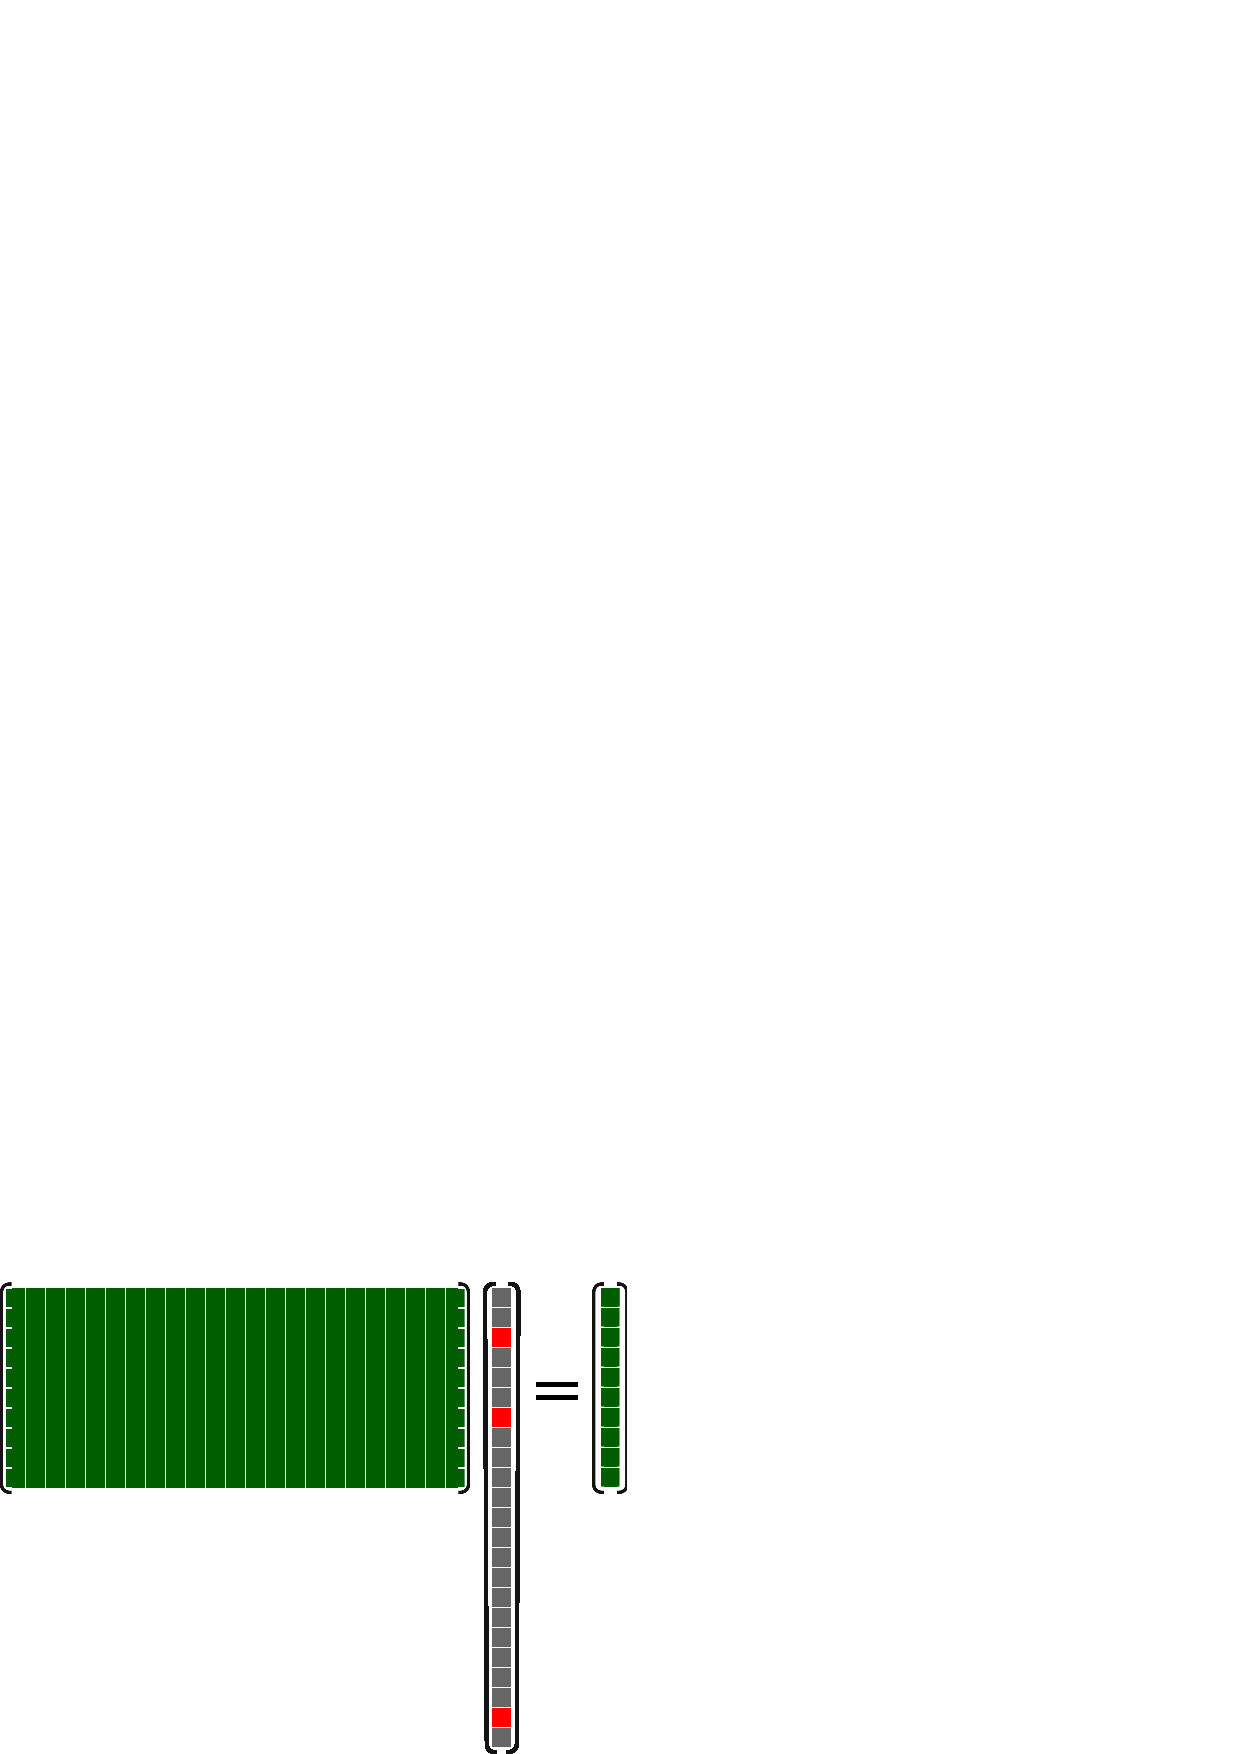
\includegraphics[width = 0.66\textwidth]{images/Da_x.pdf} % Or .pdf
\caption{Sparse Coding}
\label{fig:da_x}
\end{figure}


In the last 15 years several sparse coding algorithms have been proposed. 
Some that solve the initial problem <> greedily, the (orthogonal) matching pursuit, and others which modified the problem to become convex/linear. These primary derive from the numerical domain in the form of 
large linear system solvers with few optimization constraints. The LARS-Lasso, basis pursuit, FOCUSS?

%copy
% Following Tao et al., where it was shown that the L1 norm is equivalent to the L0 norm, 
%leads one to solve an easier problem. Finding the candidate with the smallest L1 norm can be expressed relatively
%easily as a linear program, for which efficient solution methods already exist. These solution methods have been refined over the past few years yielding enormous gain

$\lVert\alpha\rVert_{0}$ makes the problem NP-hard
to get best solution you need to test every combination
Solution:
use greedy approach 

or use $\ell_1$ as convex relaxation of $\ell_0$
the most common algorithms are the following ones.
BP/MP/OMP ...
Lasso/Ridge regression etc.

\Todo{image/description of different regularizations}


\section{$\ell_0$ regularization with greedy algorithms}

The algorithm calculates a coefficient vector $\alpha$ which is an greedy/approximate solution of the following NP-hard problem
\begin{align}
\min_{\alpha\in\mathbb{R}^{p}}  \lVert x - D\alpha \rVert^{2}_{2} \textrm{ s.t. } \lVert \alpha \rVert_{0} \leq L
\end{align}
respectivly
\begin{align}
\min_{\alpha\in\mathbb{R}^{p}}   \lVert \alpha \rVert_{0}   \textrm{ s.t. } \lVert x - D\alpha \rVert^{2}_{2} \leq \epsilon
\end{align}
\cite{Mallat1993}

\subsection{Matching pursuit}
\label{sec:mp}
\begin{algorithm}
\caption{Matching Pursuit}
\begin{algorithmic}[1]
\REQUIRE $x \in \mathbb{R}^m, y \in \mathbb{R}^m, D \in \mathbb{R}^{m\times p}$
\STATE $\alpha \gets 0, r \gets x $ (residual) 
\WHILE {$\lVert \alpha \rVert_{0} \leq L$}
\STATE Select atom with maximum correlation with residual: 
\begin{equation*}
i \gets \argmax_{i=1,...,p} \lvert d_i^Tr \rvert
\end{equation*}
\STATE update coefficients: $a[i]  \gets a[i] + d_i^Tr$
\STATE update residual: $r \gets r - \left(d_i^Tr\right)d_i$
\ENDWHILE
\RETURN $\alpha$
\end{algorithmic}
\end{algorithm}
\subsection{Orthogonal matching pursuit}
\cite{Pati1993}
\label{sec:omp}

%copy
%OMP to address the NP-hard sparse coding problem

\begin{algorithm}
\caption{Orthogonal Matching Pursuit}
\begin{algorithmic}[1]
\REQUIRE $x \in \mathbb{R}^m, y \in \mathbb{R}^m, D \in \mathbb{R}^{m\times p}, \epsilon \in \mathbb{R}$
\STATE $\alpha \gets 0, r \gets x $ (residual) $, S=\emptyset$
\FOR {$i = 1$ to $L$}
\STATE Select atom with maximum correlation with residual: 
\begin{equation*}
i \gets \argmax_{i \in S^C} \lvert d_i^Tr \rvert
\end{equation*}
\STATE update active set: $S \gets S \cup \{i\} $
\STATE update residual: $r \gets \left(I-D_S\left( D_S^T D_S \right)^{-1} D_S^T \right)x$
\STATE update coefficients: $a_S \gets \left( D_S^T D_S \right)^{-1} D_S^T x $

\ENDFOR
\RETURN $\alpha$
\end{algorithmic}
\end{algorithm}

\section {$\ell_1$ regularization}

basis pursuit\cite{} 
FOCUSS \cite{}

The LASSO (least absolute shrinkage and selection operator) is a regularized version of a least squares solution.
The regularized version is found by adding a constraint that induces the $L_1$-norm of the solution to be small. \cite{Tibshirani1998}
There are several ways to compute the LASSO. .. ...... \cite{} 

\Todo{split into LAR and LARS-lass, better illustrate than use complex formulas}
\subsection {LARS-Lasso}
\label{sec:lars}
The LARS-Lasso is a algorithm to solve the LASSO with the help of least angle regression (short LAR)
as described in \cite{Efron2004}. It is a modified version of the LAR where .... variables are removed when they cross zero ...


\begin{align}
\min_{\alpha\in\mathbb{R}^{p}}  \frac{1}{2} \lVert x - D\alpha \rVert^{2}_{2} + \lambda \lVert \alpha \rVert_{1}
\end{align}

\Todo{add algo.}
\begin{algorithm}
\caption{LARS-lasso}
\begin{algorithmic}[1]
\REQUIRE $x \in \mathbb{R}^m$
\end{algorithmic}
\end{algorithm}

\subsubsection{Limitations}
The Lasso modified version of the LAR hat the following limitations.
\begin{description}
 \item[Dimension] to high dimension of signal When the dimension $p$ of the signal $X$ is 
much higher than the the dimension $m$ of the dictionary $D$ the algorithm can only select $m$ columns.

\item[correlation] When the columns of the dictionary are highly correlated the algorithm
selects only one column.
\end{description}

Limitation one is irrelevant for our experiments as the dictionaries are over-complete 
, with respect to the dimension $m$ of signal $X$, and thus satisfy $p\leq n$.

\section{Application and Related Work}

\begin{description}
\item[noise reduction]
Remove noise from a signal. 
Using the fact that sparse coding is an approximation of signal that loses ... noise? ... in its encoding process. 
\begin{align*}
y = x + w
\end{align*}



\cite{Elad2006}

\item[in-painting]
fill missing parts by removing rows from the dictionary
Train with the original image
\begin{align*}
x \approx D\alpha\\
x_s \approx D_s\alpha\\
Wx \approx WD\alpha\text{select subset}\\
\end{align*}

\cite{mairal08sparse}

\item[compression] An example for this is the compression of facial images by Bryt and Elad \cite{Bryt2008}.
\item[classification] Examples for this can be found in \cite{Mairal2008b} and \cite{Bar2009}.

%\item[noise reduction]
%\item[in-painting]
%\item[classification] \Todo{usage:classification}

\end{description}





